\newpage
\subsection*{Обработка данных}



Стоит заметить, что определение запирающий потенциал <<на глаз>> достаточно проблематично, и, как будет показано далее, несодержательно. Поэтому запирающий потенциал находился из экстраполяции данных, считая $\sqrt{I} \sim \sqrt{U_1} \sim U_2$ (см. рис. \ref{fig:3plot}).


\begin{figure}[h]
    \centering
    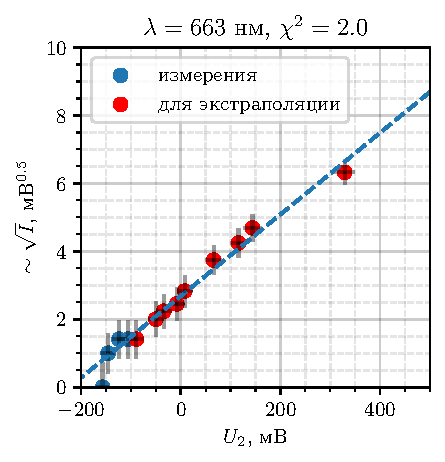
\includegraphics[width=0.3\textwidth]{figs/fig3_1.pdf}
    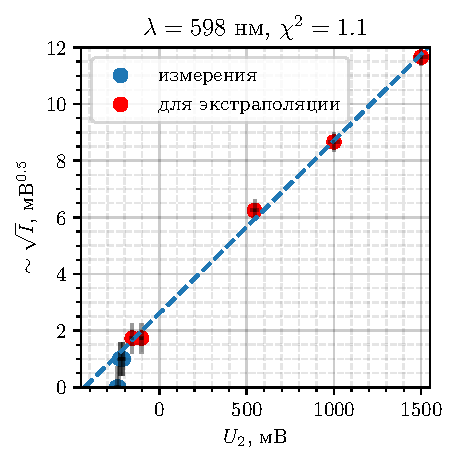
\includegraphics[width=0.3\textwidth]{figs/fig3_3.pdf}
    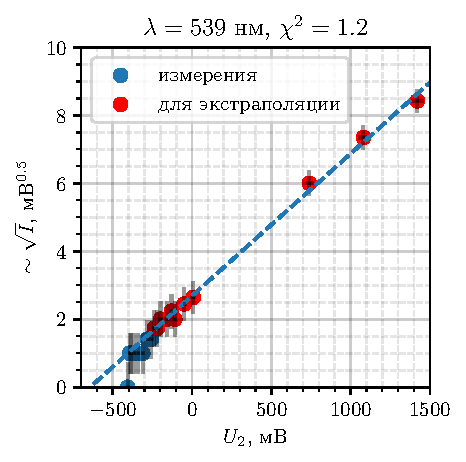
\includegraphics[width=0.3\textwidth]{figs/fig3_2.pdf}
    \vspace{-3mm}
    \caption{Экстраполяция данных, для нахождения запирающего потенциала $V_0$}
    \label{fig:3plot}
\end{figure}

Оценка $\chi^2$ лежит в диапазоне $\in [1, 2]$, что позволяет говорить об адекватности аппроксимации прямой на выбранном диапазоне и достаточности данных.

Зная $\sqrt{U_1} = a U_2 + b$, можем найти
\begin{equation*}
    V_0 = - \frac{b}{a}, 
    \hspace{5 mm} 
    \Delta V_0 = - \frac{b}{a} \left(\big|\tfrac{\Delta a}{a}\big| + \big|\tfrac{\Delta b}{b}\big|\right).
\end{equation*}
Из диагональных элементов ковариационной матрицы были оценены погрешности $a,\, b$ и, соответственно, погрешности значений для $V_0$, результаты приведены в таблице № \ref{tab:res}.


\begin{table}[h!]
    \caption{Определенные значения запирающего потенциала $V_0$}
    \centering
    \begin{tabular}{ccc}
    \toprule
        $\lambda$, нм &
        $V_0$, мВ &
        $\Delta V_0$, мВ \\ 
    \midrule
        539 &  643 & 23 \\ 
        598 &  429 & 35 \\ 
        663 &  223 & 17 \\ 
    \bottomrule
    \end{tabular}
    \label{tab:res}
\end{table}

На рис. \ref{fig:V0omega} построена зависимость $V_0 (\omega)$. 
Чтобы убедиться в несостоятельности измерений <<на глаз>>, построим значения $V_0$, измеренные на глаз. 
\vspace{-3mm}

\begin{figure}[h]
    \centering
    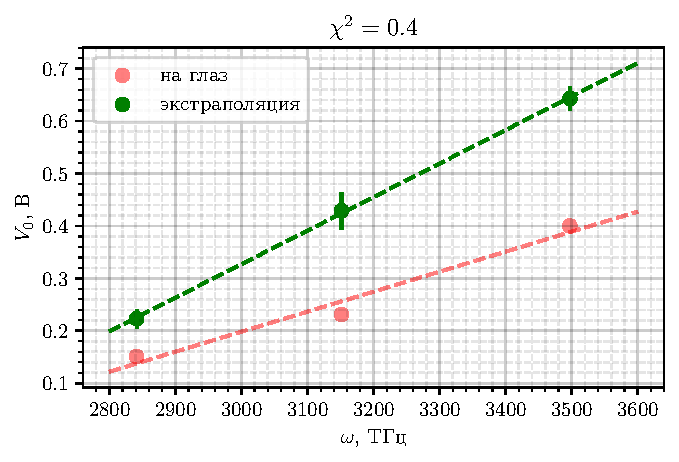
\includegraphics[width=0.5\textwidth]{figs/fig_V0.pdf}
    \caption{Зависимость $V_0 (\omega)$}
    \label{fig:V0omega}
\end{figure}

Низкое значение $\chi^2$ намекает на несостоятельность всего трёх измерений, но, с учётом разброса по $\omega$ и тому, что прямые всё же достаточно хорошо ложатся на прямую, $\xi^2 = 0.4$ не должно быть критической проблемой. 